\chapter{Fundamentos Teóricos}
Esta sección tiene el objetivo de introducir y explicar brevemente los
fundamentos teóricos en los que se basan los métodos empleados en este
proyecto, así como justificar su relevancia en la resolución del problema que
se plantea.

\subsection{Subproblemas de la IQA}
Existen tres subproblemas presenten en el ámbito de \emph{IQA}. Los primeros, son problemas 
dónde tenemos acceso a la imagen original, que suponemos exenta de desperfectos, 
en la cual se pueden aplicar métodos basados en diferencia de características 
entre ambas, como puede ser al nivel del color de píxel posición a posición,
y se denomina ``\emph{Full Reference}''(\emph{FR}). 
La tarea, aparentemente sencilla, en realidad presenta una complejidad alta dada por 
la necesidad de codificar la percepción humana a la hora de calificar la calidad 
de una imagen\cite{WhyIsIQASoDifficult}. Ya que métricas que miden distancias no suelen ser suficientes, 
ver imágenes~(\ref{fig:FailureMinkowskiMetric},\ref{fig:MSEHyperSphere}).

\Enrique[{Hablar de las limitaciones de métricas de distancias} ]{ Pequeño párrafo sobre estas limitaciones }
 
Los segundos son aquellos dónde tenemos algún tipo de información adicional respecto 
a la imagen original en el momento de asesoramiento de la calidad de la imagen final,
denominados ``\emph{Reduced Reference}''(\emph{RR}). La información extra puede incluir características estadísticas, metadatos, parámetros 
de compresión o características extraídas de una región de interés específica.
 
Y por último, tenemos aquellos problemas donde desconocemos el origen y cualquier 
información respecto a la imagen inicial, denominados problemas ``\emph{No reference}''(\emph{NR}).
Estas métricas están exentas de cualquier información de referencia y se 
centran en capturar características generales de calidad. 

\Enrique[{Enfatizar las diferencias en dificultad FR NR}]
{Parrafo sobre las dificultades FR - NR extendiendo la extraccion de caracteristicas de NR}

La complejidad del problema crece conforme nos desplazamos a las tres dimensiones. 
El analizar la calidad de los modelos \emph{3D} implica mayor nivel de dificultad 
dado que nos enfrentamos a dos grandes retos: La complejidad computacional 
de las operaciones y la escasez de bases de datos etiquetadas
sobre objetos tridimensionales para entrenar y evaluar modelos. 
 
Para las nubes de puntos, que representan una colección de puntos en un espacio 
tridimensional $(x,y,z)$ cada uno con un color asociado \emph{RGB}, se pueden emplear métricas y algoritmos basándose en criterios como la 
densidad de puntos, la uniformidad, la precisión geométrica y la detección de artefactos.
También se pueden considerar aspectos relacionados con la coherencia de los colores 
o texturas asociadas a los puntos\cite{NR3DQA, StructureGuidedResampling, GPA-NET} 
 
Un enfoque común es la evaluación de calidad de una nube de puntos tridimensional 
mediante proyecciones \emph{2D} desde diferentes perspectivas\cite{IT-PCQA, VQA-PC, MM-PCQA}. 
De esta forma podemos tratar el problema como uno de \emph{IQA} 2D reduciendo la 
complejidad computacional, pudiendo implementar métodos y soluciones ya existentes.

Teniendo en cuenta todas estas consideraciones, el presente TFG aborda la
estimación, sin referencia, de calidad de imágenes médicas en espacio tridimensional.

\begin{figure}[htp]
  \begin{center}
    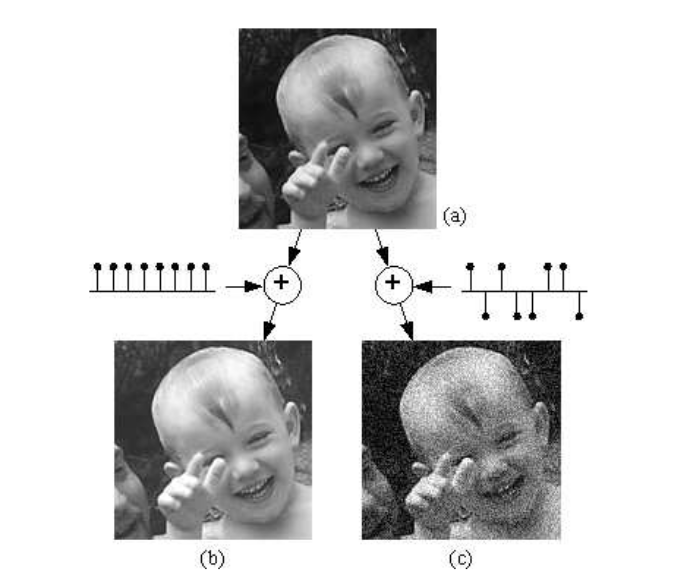
\includegraphics[width=0.5\textwidth]{imagenes/chapter1/failure_minkowski_metric.png}
  \end{center}
  \caption{En este ejemplo, extraído de\cite{MinkowskiFailure},
  vemos que sumar una constante positiva a una imagen  de referencia (a) produce la imagen (b) que contiene la misma distancia \emph{Minkowski}\footnotemark[1]
  que (c), imagen fabricada por la misma constante pero permutando signo de forma aleatoria. Siendo que
  la percepción final es que la imagen (c) es peor que la (b).
\label{fig:FailureMinkowskiMetric}}
\end{figure}
\begin{figure}[htp]
  \begin{center}
    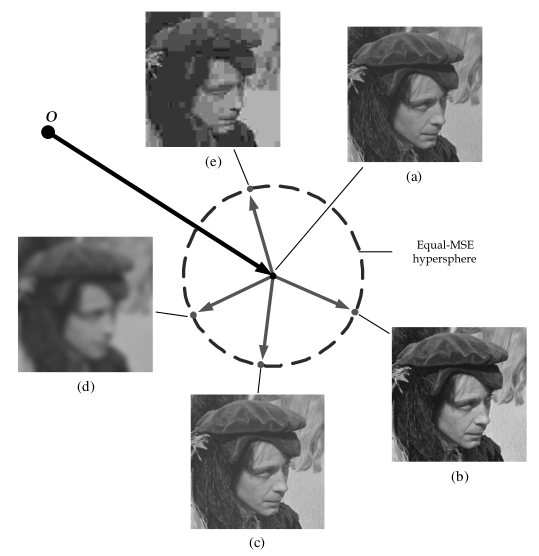
\includegraphics[width=0.5\textwidth]{imagenes/chapter1/MSE_Hypersphere.png}
  \end{center}
  \caption{En este ejemplo, extraído de\cite{Wang2006ModernIQ}, la misma imagen distorsionada de distintas maneras
  resulta en el mismo valor \emph{MSE}\footnotemark[2]=181. Siendo evidente que 
  algunas distorsiones producen efectos visuales más marcados que otras haciendo 
  que no sea una buena estimación perceptual de la calidad.}
  \label{fig:MSEHyperSphere}
\end{figure}

\footnotetext[1]{La distancia de \emph{Minkowski} es una métrica 
vectorial que puede considerarse como una generalización tanto de 
la distancia euclidia como de la distancia de Manhattan . }
\footnotetext[2]{\emph{MSE}: \emph{Mean squared error} o error cuadrático medio 
  es una métrica de distancia que se calcula como la media de la suma de las 
  diferencias al cuadrado.}

\section{Aprendizaje Automático}
El aprendizaje automático\cite{IAModernApproach} o \emph{MachineLearning} (\emph{ML}) 
es una de las ramas que compone lo que definimos como 
la inteligencia artificial (\emph{IA}). Esta última se puede definir, 
según\cite{WhatIsAI}, como 
``La ciencia e ingeniería 
de crear máquinas inteligentes, especialmente programas de computadora inteligentes. 
Está relacionada con la tarea similar de utilizar computadoras para comprender 
la inteligencia humana...''

En este caso hablamos de dar soluciones a problemas complejos sin 
solución analítica (o que resulta muy costoso hallarla), es decir, necesitamos que la computadora sea la que identifique
los patrones en los datos y realice predicciones sobre ellos\cite{LearningFromData}.
Se puede definir más formalmente que un programa aprende de la experiencia E con
respecto a alguna clase de tareas T y una métrica de rendimiento P si su
rendimiento en las tareas T, medido con P, mejora con la experiencia E\cite{TomMitchell}.

Dependiendo de factores como las necesidades del problema, la naturaleza
de los datos a utilizar o el objetivo a alcanzar, podemos encontrar distintos tipos de
algoritmos de aprendizaje. En este documento se recogerán dos grandes grupos: aprendizaje supervisado 
y aprendizaje no supervisado. En el primero disponemos de un conjunto de datos 
anotados, es decir, con las salidas deseadas para cada ejemplo y en el segundo 
se espera que sea la máquina la que determine los patrones~(\ref{fig:MLExamples}). 

En general se suelen aplicar las técnicas de \emph{ML} sobre grandes conjuntos 
de datos sobre los cuales deseamos detectar los patrones subyacientes\cite{
DataMiningHandbook}.

Puede observarse que dada estas descripciones, al problema presente podemos 
aplicarle alguna técnica de \emph{ML}: Tenemos datos de entrada (nubes de puntos 
distorsionadas) y una salida (valor de calidad). Además, existen conjuntos de 
datos públicos etiquetadas para distintos tipos de distorsiones. Esto significa que
estamos entre un problema de aprendizaje supervisado.


\begin{figure}[htp]
  \begin{center}
    \subfloat{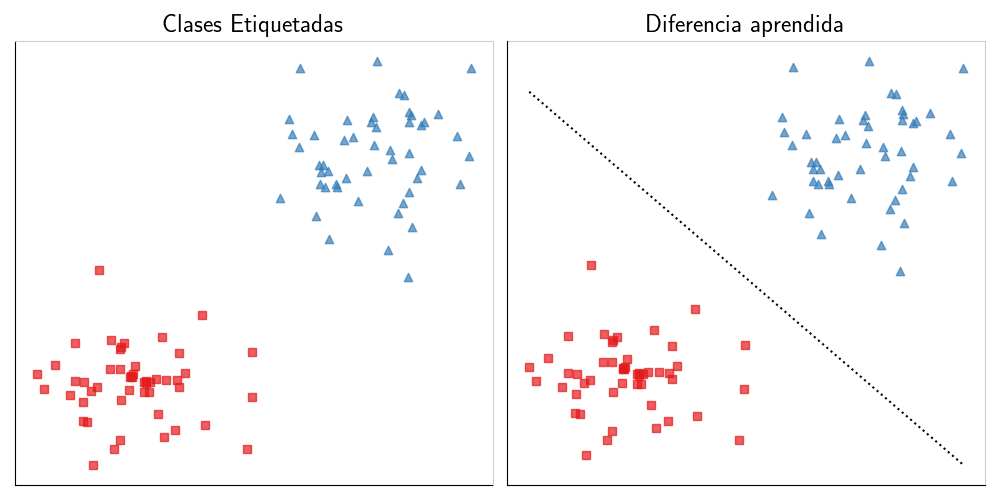
\includegraphics[width=0.85\textwidth]{imagenes/chapter2/SVMExample.png}}\\ 
    \subfloat{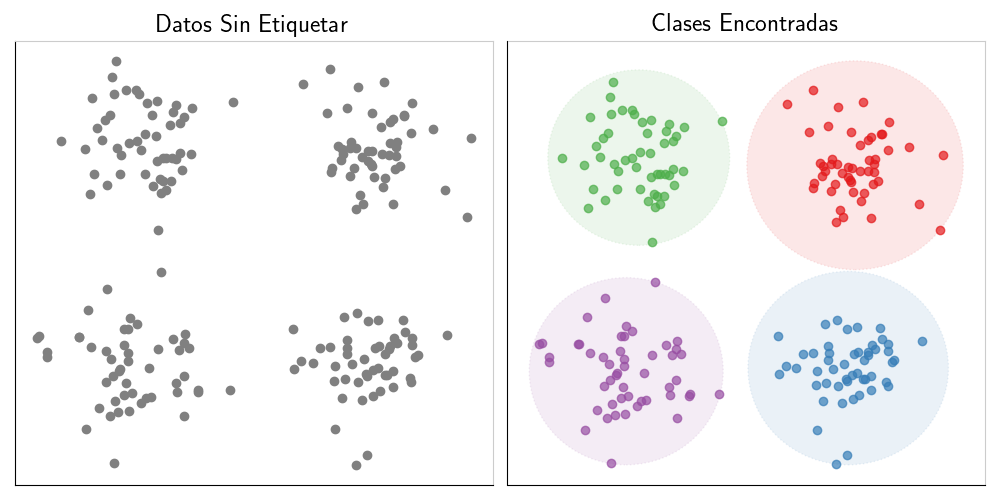
\includegraphics[width=0.85\textwidth]{imagenes/chapter2/ClusteringExample.png}}
  \end{center}
  \caption{Ejemplo de aprendizaje supervisado y no supervisado. En el primer par, 
  vemos como dado un conjunto de clases etiquetadas aprendemos un hiper plano que 
  las separa. En el segundo, dado un conjunto de puntos aprendemos un conjunto de clases.
}
  \label{fig:MLExamples}
\end{figure}

\section{Aprendizaje Profundo}
El aprendizaje profundo o \emph{Deep Learning} (\emph{DL}) 
\subsection{Redes Convolucionales} 
\subsection{Aplicadas a Videos} 
\section{Ensemble o Conjunto \emph{Deep Learning}}
\section{Imágenes médicas, Métricas y Distorsiones}
\label{sec:Distorsiones}
